\documentclass[letterpaper,11pt]{article}
\usepackage{graphicx}
\usepackage{listings}
\usepackage[super]{nth}
\usepackage[hyphens]{url}
\usepackage{hyperref}
\usepackage{amsmath}
\usepackage[makeroom]{cancel}
\usepackage[table]{xcolor}
\usepackage{comment}
\usepackage[space]{grffile}
\usepackage{csvsimple}
\usepackage{longtable}


\newcommand*{\srcPath}{../src}%

\lstset{
	basicstyle=\footnotesize,
	breaklines=true,
}

\begin{document}

\begin{titlepage}

\begin{center}

\Huge{Assignment 9}

\Large{CS 532:  Introduction to Web Science}

\Large{Spring 2017}

\Large{Grant Atkins}

\Large Finished on \today

\end{center}

\end{titlepage}

\newpage


% =================================
% First question
% =================================
\section*{1}

\subsection*{Question}

\begin{verbatim}
1.  Choose a blog or a newsfeed (or something similar with an Atom
or RSS feed).  Every student should do a unique feed, so please
"claim" the feed on the class email list (first come, first served).
It should be on a topic or topics of which you are qualified to
provide classification training data.  Find something with at least
100 entries (or items if RSS).

Create between four and eight different categories for the entries
in the feed:

examples: 

work, class, family, news, deals

liberal, conservative, moderate, libertarian

sports, local, financial, national, international, entertainment

metal, electronic, ambient, folk, hip-hop, pop

Download and process the pages of the feed as per the week 12 
class slides.

Be sure to upload the raw data (Atom or RSS) to your github account.
\end{verbatim}

\clearpage
\subsection*{Answer}

For this problem I decided to use Realm's RSS feed, a news feed for mobile development \cite{realmref}. I had 7 categories to classify this feed which were: iOS, Android, React Native, Realm News, Databases, Nodejs and Xamarin. These categories mostly describe the topics that were found in these news feeds. Realm News was used to describe topics that weren't particularly programming fields or platforms but just generic news topics. Realm's RSS feed originally had approximately 700 items, I decided to take the most recent 100 items with the full list shown in my github repository \cite{github}. The 100 items used in this assignment are shown in Listing \ref{}. One thing I noticed before starting the subsequent problems was that a lot of the descriptions used common terms but in different context. For example, ``Reactive programming'' is not a synonym for ``React Native'' which was a programming language, this lead me to think that the classifier would later get these categories wrong frequently.

To get Realm's RSS feed I used the methods created in \textbf{getFeed.py}. The manual classification of the 100 RSS feed items was created in a seperate text file called \textbf{classifiedFeeds.txt}. This was used later for speeding up running the python script.

\begin{table}[htb]
\centering
\begin{tabular}{ | l | l |}
\hline
\textbf{Item Title} & \textbf{Actual Category} \\
\hline
Everyday Reactive & React Native \\ 
Providing Better Feedback in Realtime Object Detection Apps & iOS \\ 
Fragments: The Solution to (and Cause of) All of Android's Problems & Android \\ 
Realm ObjC \& Swift 2.6: Async Open Realm, Admin Flag, Compact On Launch \& Bug Fixes! & iOS \\ 
Building a Gantt Chart from Github Issues: With Near Caching Using Realm & Realm News  \\ 
Building Your Own Tools & React Native  \\ 
Server-Side Swift Live Coding & iOS  \\ 
Legal Risks and Rights for Developers & Realm News  \\ 
The Post-MVC Age & React Native \\ 
Making Mock Objects More Useful & iOS \\ 
Exploring New Android Layouts & Android \\ 
Crafting Collaborative Apps with Realm & Realm News \\ 
Visual Studio Code: Shipping One of the Largest Microsoft JavaScript Apps & Xamarin \\ 
Swift on Android: The Future of Cross-Platform Programming or White Whale? & Android \\ 
Realm Java 3.1: Object Notifications, Backup Recovery and Reverse Relationships & Android \\ 
Reverse Engineering Is Not Just for Hackers & Android \\ 
Git at Scale: Managing Swift/Obj-C Code \& Coders & iOS \\ 
Realm World Tour: That’s a Wrap Time for Round Two! & Realm News \\ 
Swift's Pointy Bits: Unsafe Swift \& Pointer Types & iOS  \\ 
Tutorial: Build iOS App from Scratch & iOS  \\ 
Realm ObjC \& Swift 2.5: Query Improvements, Swift 3.1 Binaries \& Bug Fixes! & iOS\\ 
Data Binding in the Real World & Android \\ 
Taming Node_Modules at Facebook & Nodejs \\ 
The Safety of Unsafe Swift & iOS \\ 
Realm Browser Tutorial & Realm News \\ 
Scaling Open Source Communities & Realm News \\ 
Evolution in Action: Software Architecture as Systems Dissolve & Realm News \\ 
Bring Your Own Authentication: Connect Your Users to the Realm Mobile Platform & Realm News \\ 
No More Typos: Foolproof Notifications in Swift & iOS \\ 
Getting Down to Business With Firebase Monitoring Tools & Databases \\ 
Making PostgreSQL Realtime & Databases \\ 
Everything You Ever Wanted To Know About Sequence and Collection & iOS \\ 
Building a Blog with Realm Node.js and Express & Nodejs \\ 
Apple and VR & iOS \\ 
Espresso: Beyond the Basics & Android  \\ 
Break the Monolith with (B)Viper Modules & iOS \\ 
UI and Snapshot Testing & iOS \\ 
Scaling Your App for Rapid Growth by using Testing, Deploying and Monitoring & Xamarin \\ 
Realm Everywhere, with JavaScript: Announcing Universal Node.js Support & Nodejs \\ 
Revisiting Types in Kotlin & Android \\ 
Realm Primary Keys Tutorial & Databases \\ 
Integrating Azure Authentication with Realm & Xamarin \\ 
Hacking SiriKit & iOS \\ 
Test Driven Development (TDD) for the Masses & iOS \\ 
VoiceOver is Awesome & iOS \\ 
Interacting with Your App Through the Command Line & Android \\ 
Realm Java 3.0: Collection Notifications, Snapshots and Sorting Across Relationships & Android \\ 
Swift at Scale & iOS \\ 
Playgrounds: teach nerdy stuff in a fun and efficient way! & iOS \\ 
Sell Out and Save the World! & Realm News \\ 
Testing Functional Reactive Programming Code & iOS \\ 
Functional on Android: Lambdas, Rx, and Streams in Your App & Android \\ 
Pushing the Boundaries of Swift to the Server & iOS \\ 
Stylish Developers Guide to Unit Testing in Swift & iOS \\ 
The History of Mac and iOS: Squirrels, Disco, and Nate Eror & iOS \\ 
Selling Your Weird Mouth Noises & Realm News \\ 
Acceptance Testing & iOS \\ 
RxJava for the Rest of Us & Android \\ 
Realm + Microsoft: Xamarin, Azure, and Windows Desktop & Xamarin \\ 
Data Consistency in an Unpredictable World & iOS \\ 
Network Testing & iOS \\ 
Be the Quality You Want to See in Your App [Swift edition] & iOS \\ 
The 2016 Android Developer Toolbox & Android \\ 
Realm Cocoa Tutorial: Encryption with Realm & iOS \\ 
MVVM with Coordinators and RxSwift & iOS \\ 
Visualize, Document, and Explore Your Software Architecture & Realm News \\ 
How Indies Can Still Impact the Future of iTunes & Realm News \\ 
Realm React Native 1.0: Powerful Object Database Meets the Realm Mobile Platform & React Native \\ 
Creating the Future & iOS \\ 
Compile Time Errors Are Good & iOS \\ 
Better Android Development with Kotlin \& Gradle & Android \\ 
Realm: How I Learned to Love Databases Again & Databases \\ 
Operators and Strong Opinions & iOS \\ 
Realm ObjC \& Swift 2.4: Object Notifications! & iOS \\ 
A Startup’s Secret Weapon: The Product Engineer & Realm News \\ 
Testing an Untested App & iOS \\ 
Writing Software to Make a Difference & Realm News \\ 
Radical Hospitality - One Shower at a Time & Realm News \\ 
MVC vs. MVP vs. MVVM on Android & Android \\ 
Bringing the Platform Experience to You: Announcing the Realm World Tour & Realm News \\ 
The Objective-C Runtime \& Swift Dynamism & iOS \\ 
Reactive Apps: How to Build More Engaging Mobile Experiences & Realm News \\ 
Mastering Realm Notifications & iOS \\ 
Event Handling in the Realm Object Server & Realm News \\ 
A Designer’s Response to Silicon Valley & Realm News \\ 
Ready for Realtime and Scale: Announcing Realm Mobile Platform 1.0 & Realm News \\ 
Eventually Consistent: How to Make a Mobile-First Distributed System & Realm News \\ 
Realm ObjC \& Swift 2.3: Sync Progress Notifications, Improved Sharing \& Backup Recovery! & iOS \\ 
Realm Java 2.3: Improved Sharing, Backup Recovery and Wildcard Queries & Android \\ 
Smoke \& Mirrors: The Magic Behind Wonderful UI in Android & Android \\ 
% TEST SET STARTS HERE
JP Simard on Realm \& Open Source on the Consult Podcast & Realm News \\ 
Testing in Swift: Protocols \& View Models & iOS \\ 
Property-Based Testing with SwiftCheck & iOS \\ 
Realm Objective-C \& Swift 2.2: Objects across threads, sort over relationships \& more! & iOS  \\ 
Contextual Communication in a Connected World & Realm News \\ 
Introduction to Xamarin Forms Custom Renderers & Xamarin \\ 
Modern Android: Ditching Activities and Fragments & Android  \\ 
Safe vs Deep Integration of Realm & Android \\ 
Watch Your Language!: The Road to Cleaner Code with SwiftLint & iOS \\ 
Introducing the Realm Mobile Platform & Databases \\ 
\hline
\end{tabular}
\caption{}
\label{table:q1csvtable}
\end{table}



% \clearpage
%  \begin{figure}[h]
%  \centering
%  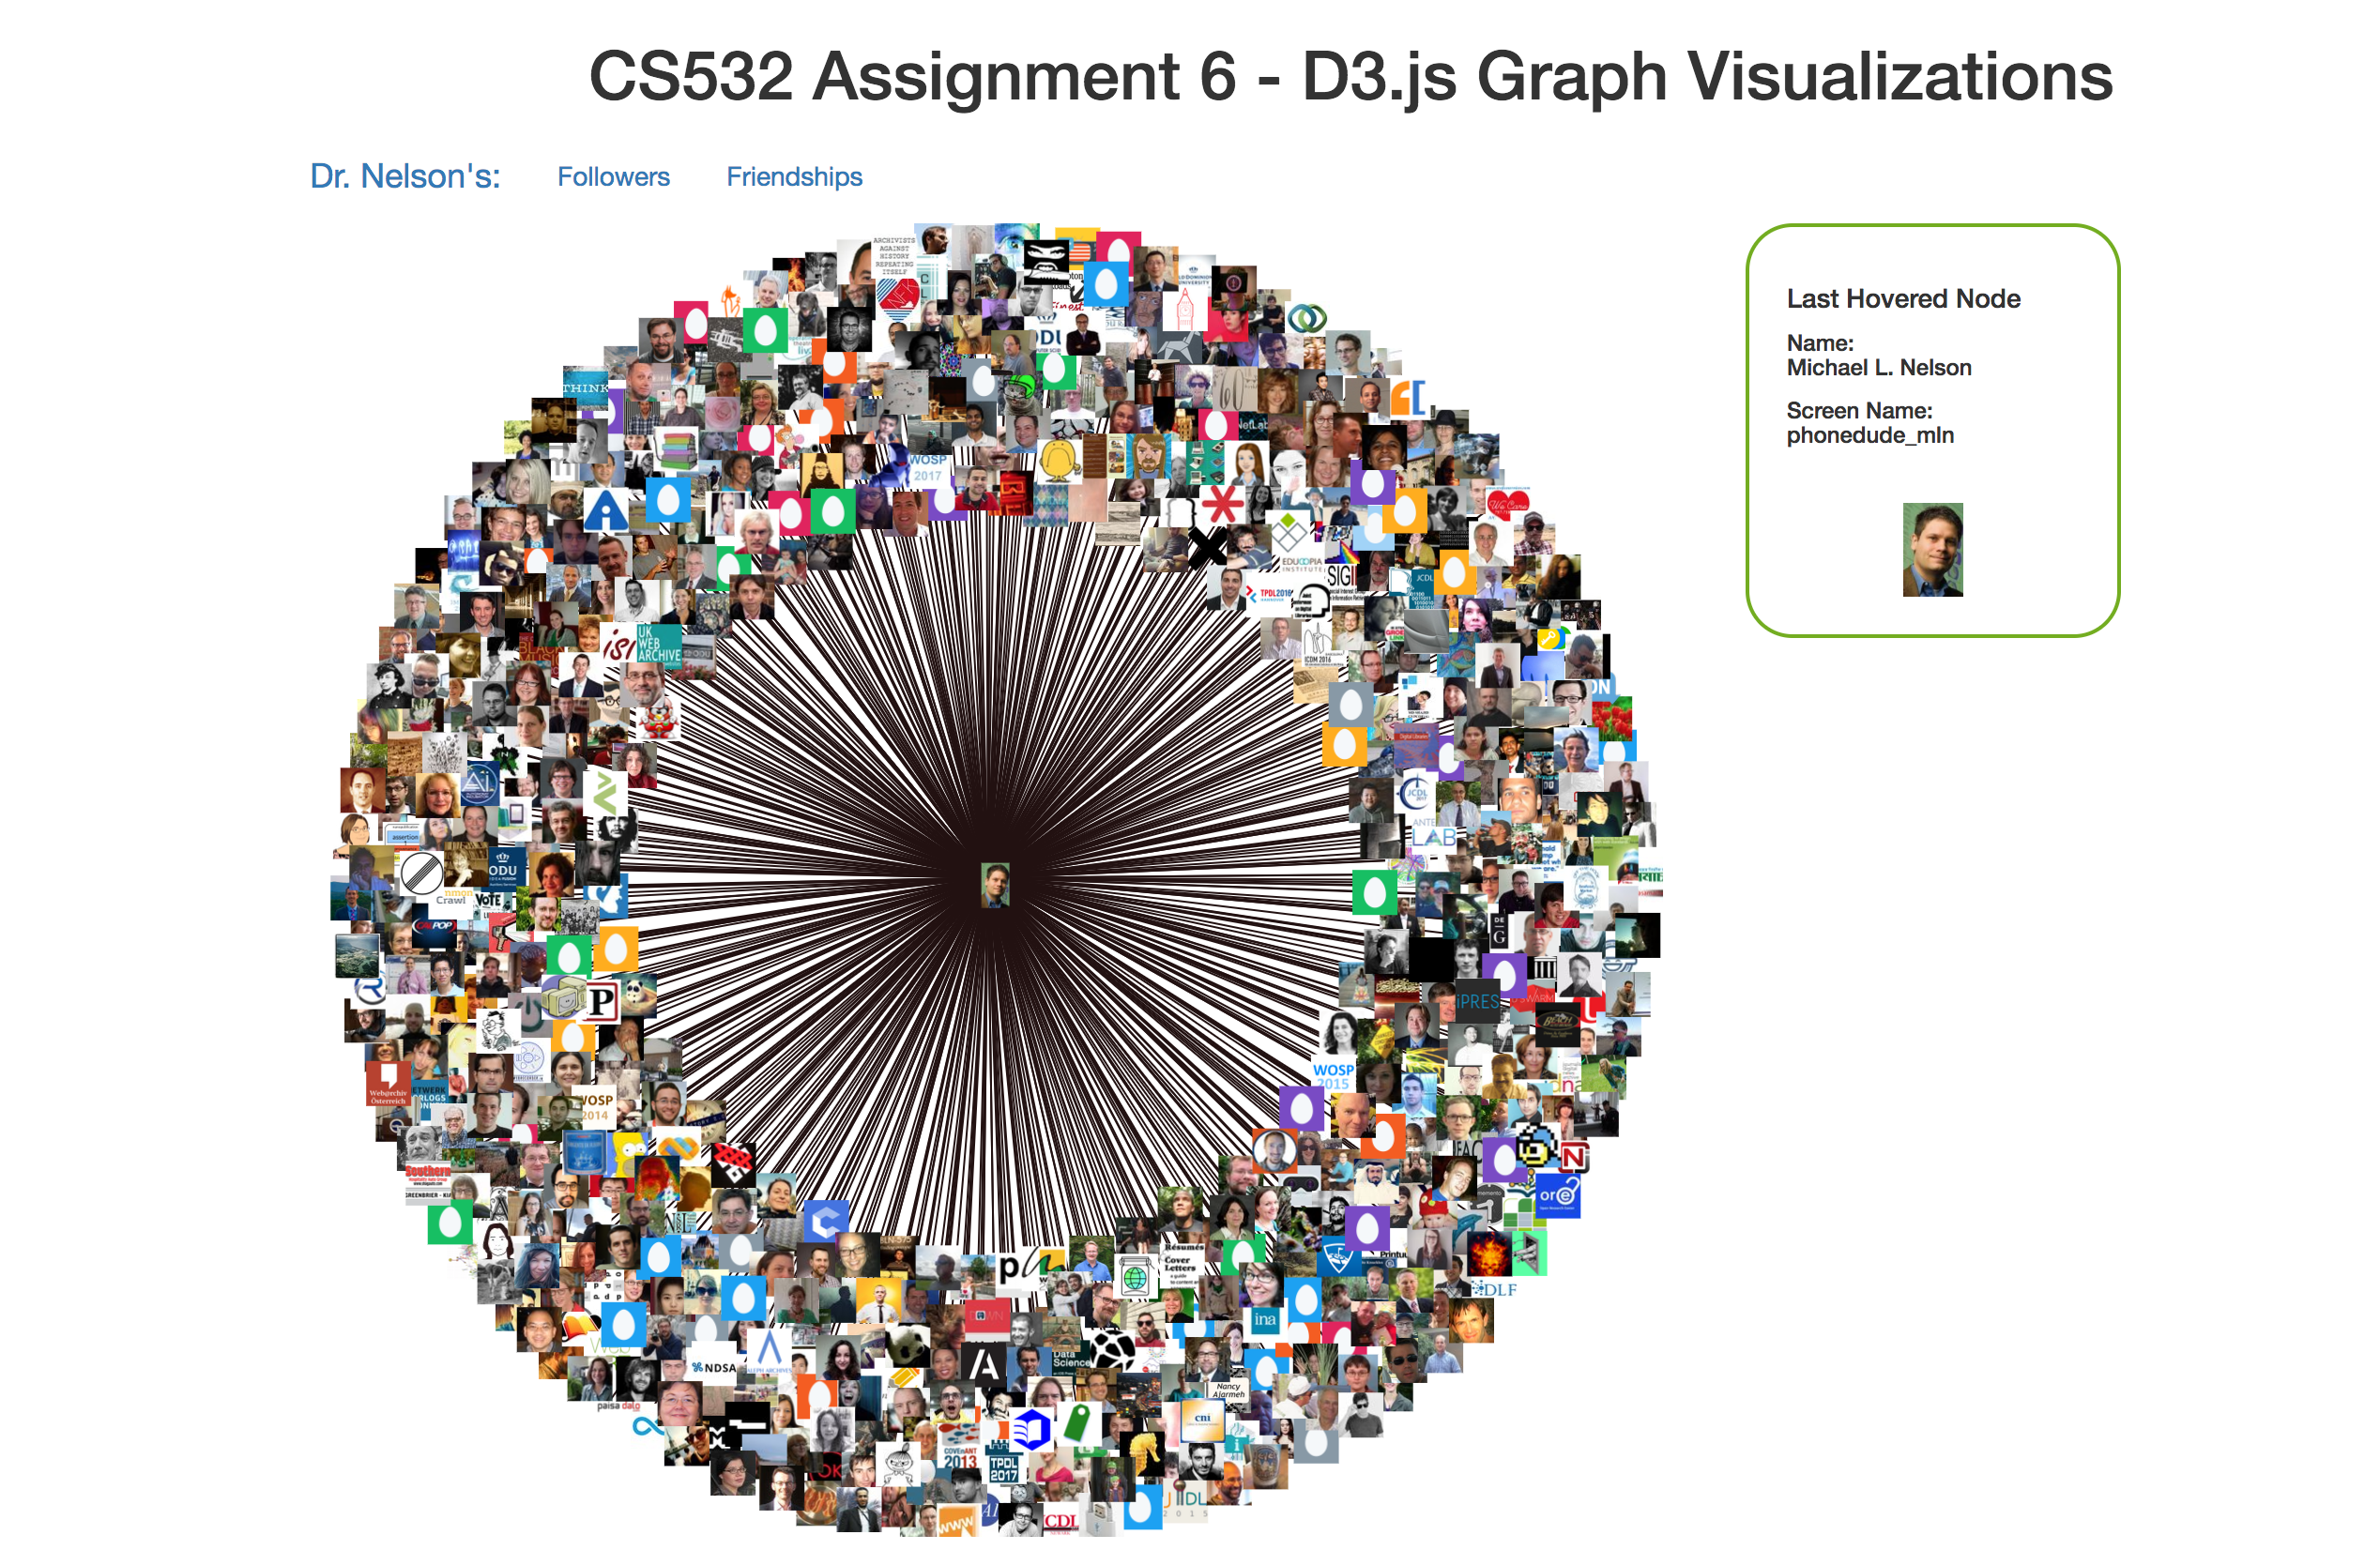
\includegraphics[scale=0.4]{d3followerGraph.png}
%  \caption{All of Dr. Nelson's followers in D3 force directed graph}
%  \label{fig:q1friendshipgraph}
%  \end{figure}


\clearpage

% =================================
% Second question
% =================================

\section*{2}

\subsection*{Question}

\begin{verbatim}
2.  Train the Fisher classifier on the first 50 entries (the "training
set"), then use the classifier to guess the classification of the
next 50 entries (the "test set").

Assess the performance of your classifier in each of your categories
by computing precision, recall, and F-measure.  Use the "macro-averaged"
label based method, as per:

http://stats.stackexchange.com/questions/21551/how-to-compute-precision-recall-for-multiclass-multilabel-classification

For example, if you have 5 categories (e.g., 80s, metal,
alternative, electronic, cover), you will compute 
precision, recall, and F-measure for each category,
and then compute the average across the 5 categories.
\end{verbatim}

\subsection*{Answer}

To solve this I used the python code provided from the Programming Collective Intelligence book described in the files \textbf{docclass.py} and \textbf{feedfilter.py}. I had to slightly modify docclass's first dependency to compile in python 3. I altered feedfilter's code heavily, creating new dictionaries for each of the classifier's guesses and actual answers as shown in Listing \ref{lst:q1feedfilter}. Feedfilter extracted the title and description from each item in the RSS feed and would concatenate the two which would then be used for classifying and training, if the iteration count was lower than the desired train count which was defined as \textit{trainCount}. Realm's RSS feed also had some items with quotation marks, emoji icons and img html tags. To compensate for this, I created two methods \textit{remove_emojis} and \textit{remove_img_tags} which removed these unwanted items before guessing or training based on the text.


% \begin{figure}[h]
% \centering
% 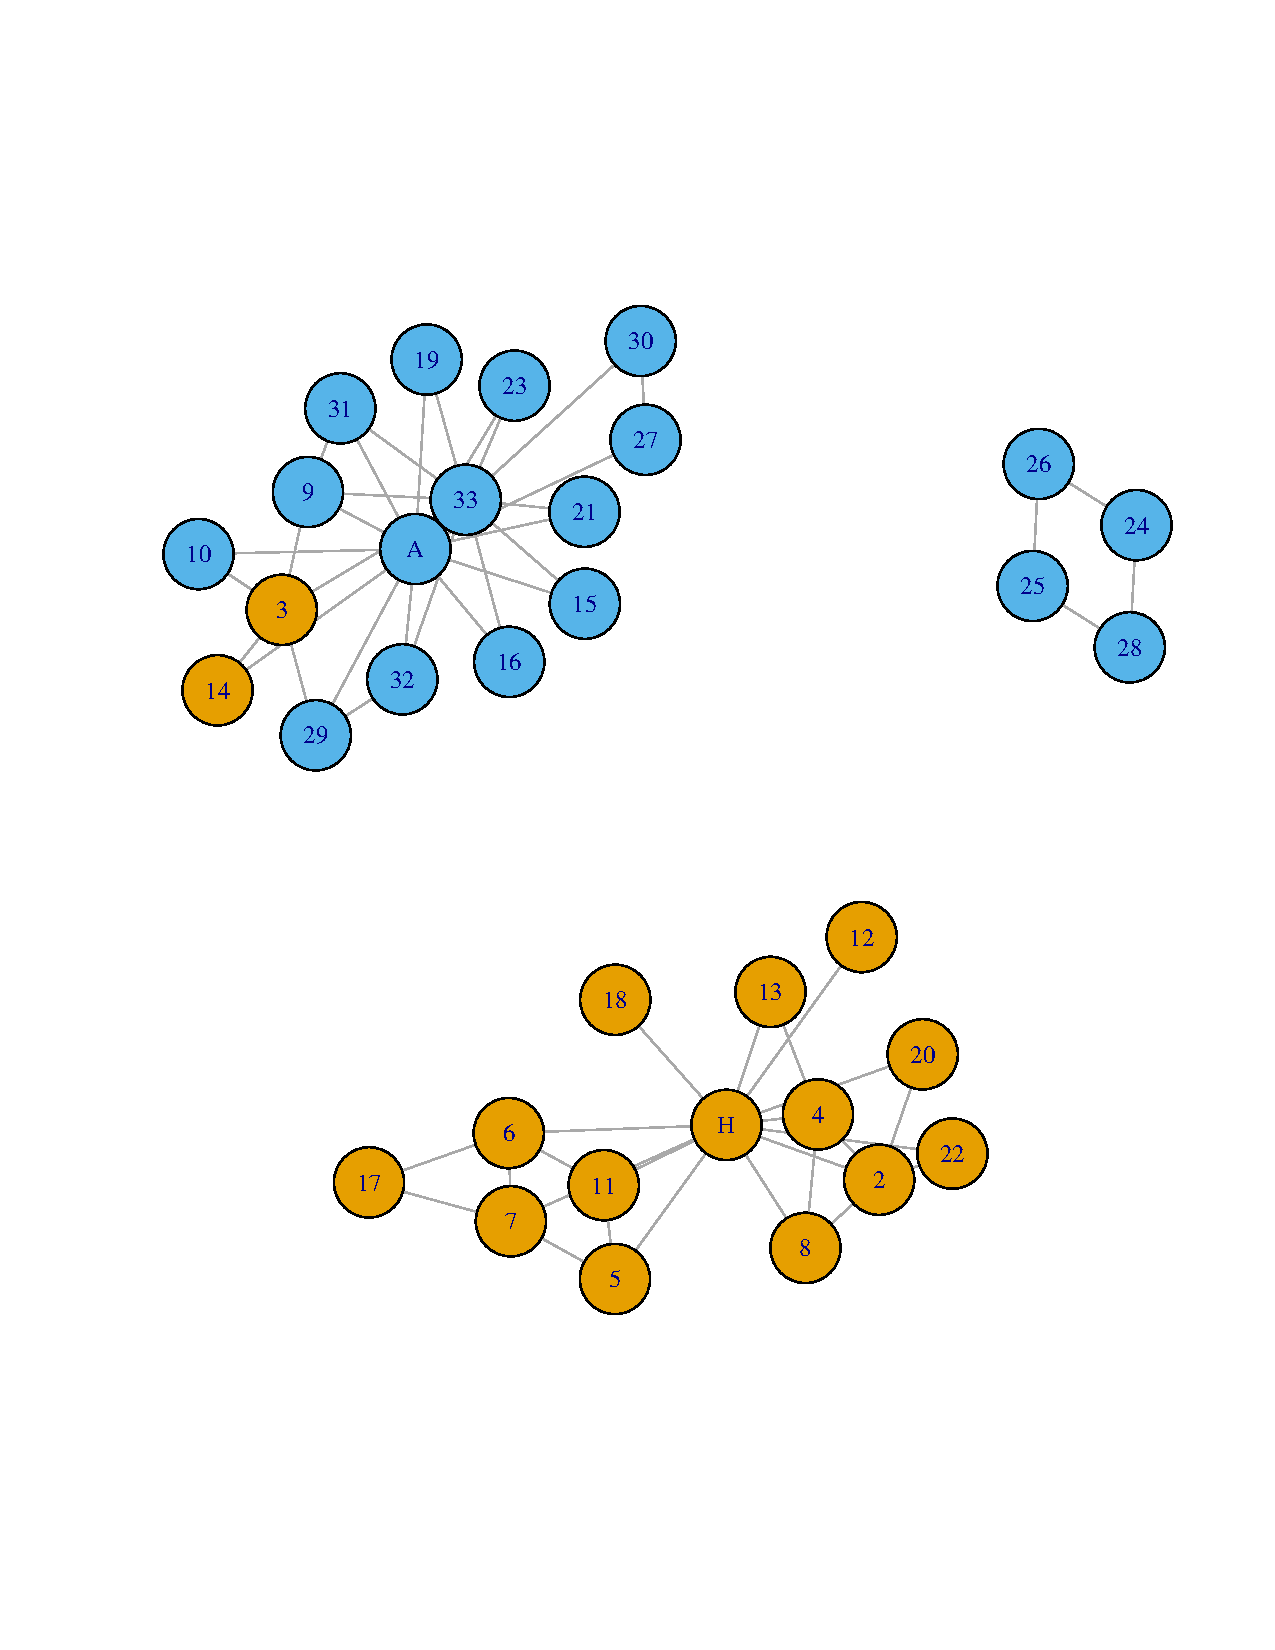
\includegraphics[scale=0.6]{predictedSplit3.pdf}
% \caption{Group split of 3 with Girvan-Newman algorithm from karateClub.R}
% \label{fig:split3}
% \end{figure}

\clearpage

% =================================
% 3rd question
% =================================

\section*{3}

\subsection*{Question}

\begin{verbatim}
3.  Repeat question #2, but use the first 90 entries to train your
classifier and the last 10 entries for testing.
\end{verbatim}

\subsection*{Answer}

\begin{center}
\Huge{NOT ATTEMPTED}
\end{center}

% \begin{figure}[h]
% \centering
% 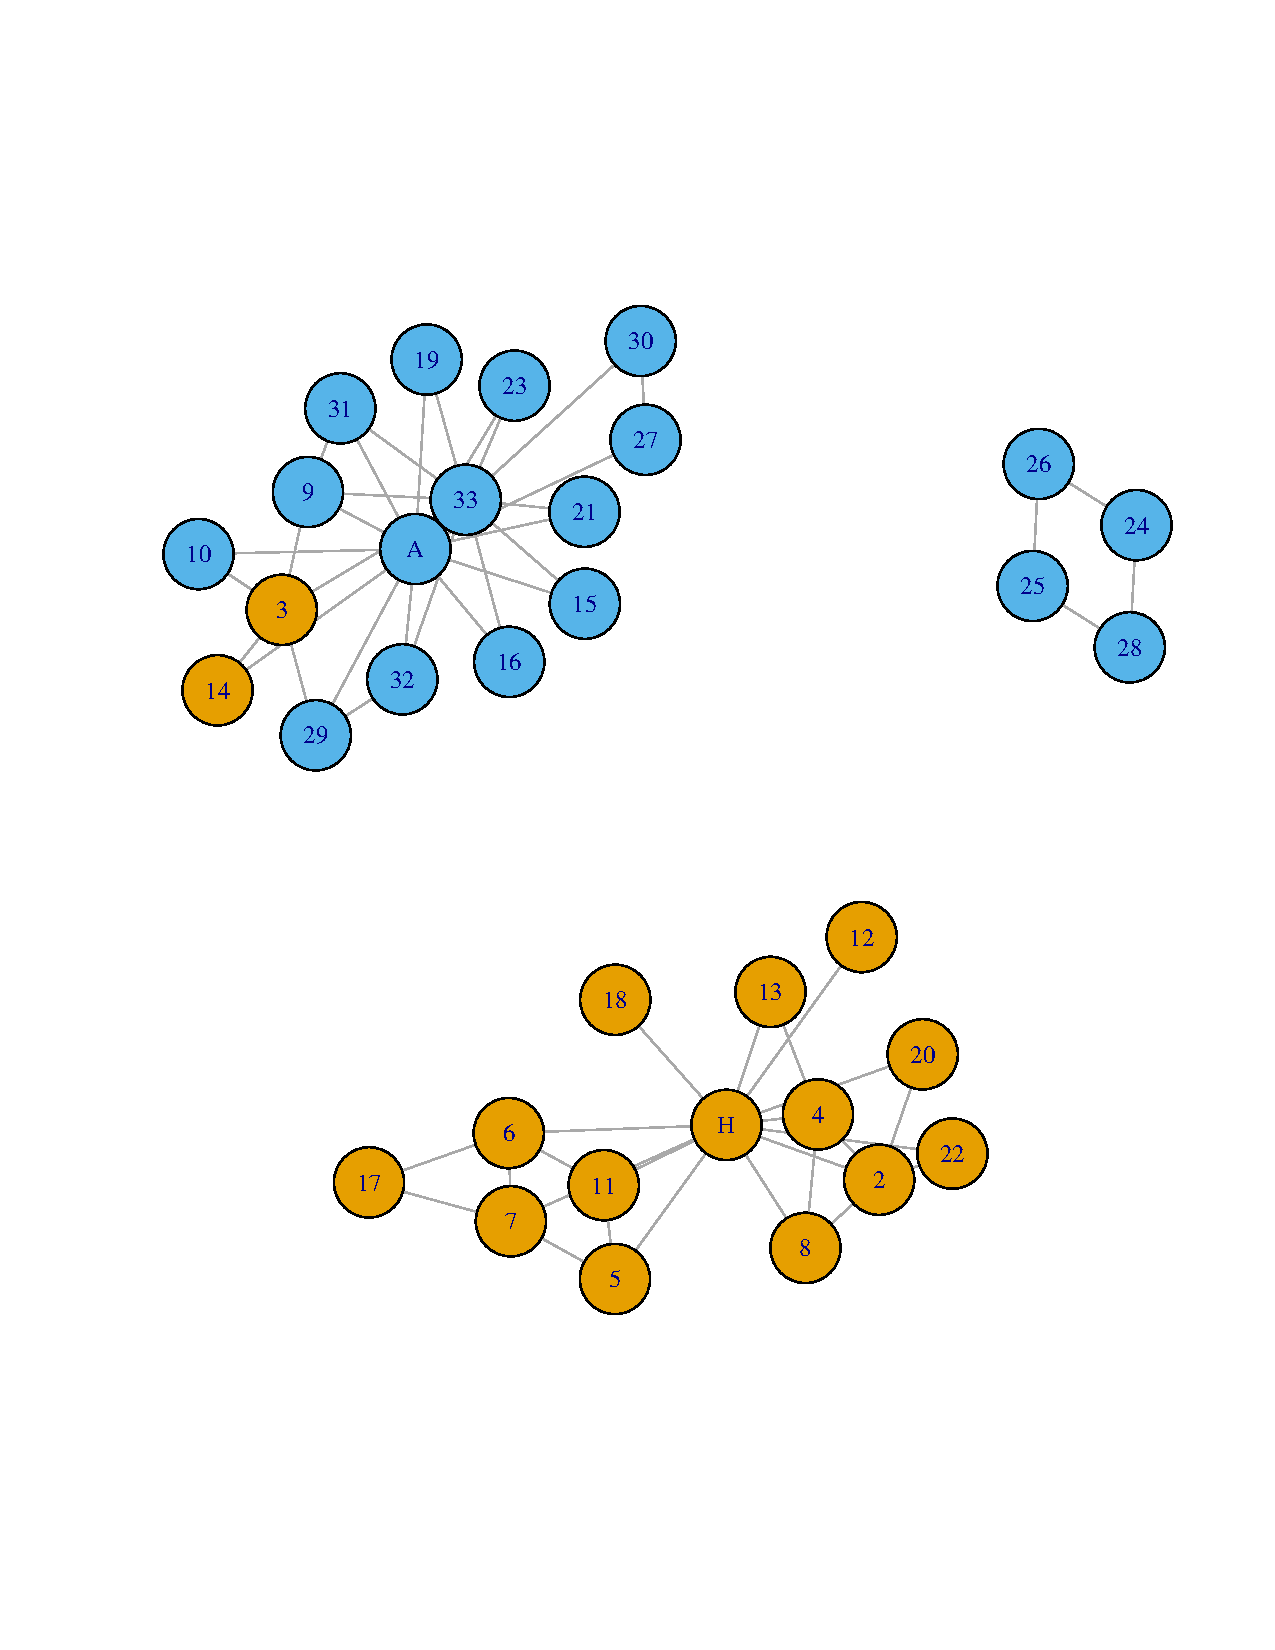
\includegraphics[scale=0.6]{predictedSplit3.pdf}
% \caption{Group split of 3 with Girvan-Newman algorithm from karateClub.R}
% \label{fig:split3}
% \end{figure}


% =================================
% 4th question
% =================================

\section*{4}

\subsection*{Question}

\begin{verbatim}
4.  Rerun question 3, but with "10-fold cross validation".  What
was the change, if any, in precision and recall (and thus F-Measure)?
\end{verbatim}

\subsection*{Answer}

\begin{center}
\Huge{NOT ATTEMPTED}
\end{center}

% \begin{figure}[h]
% \centering
% 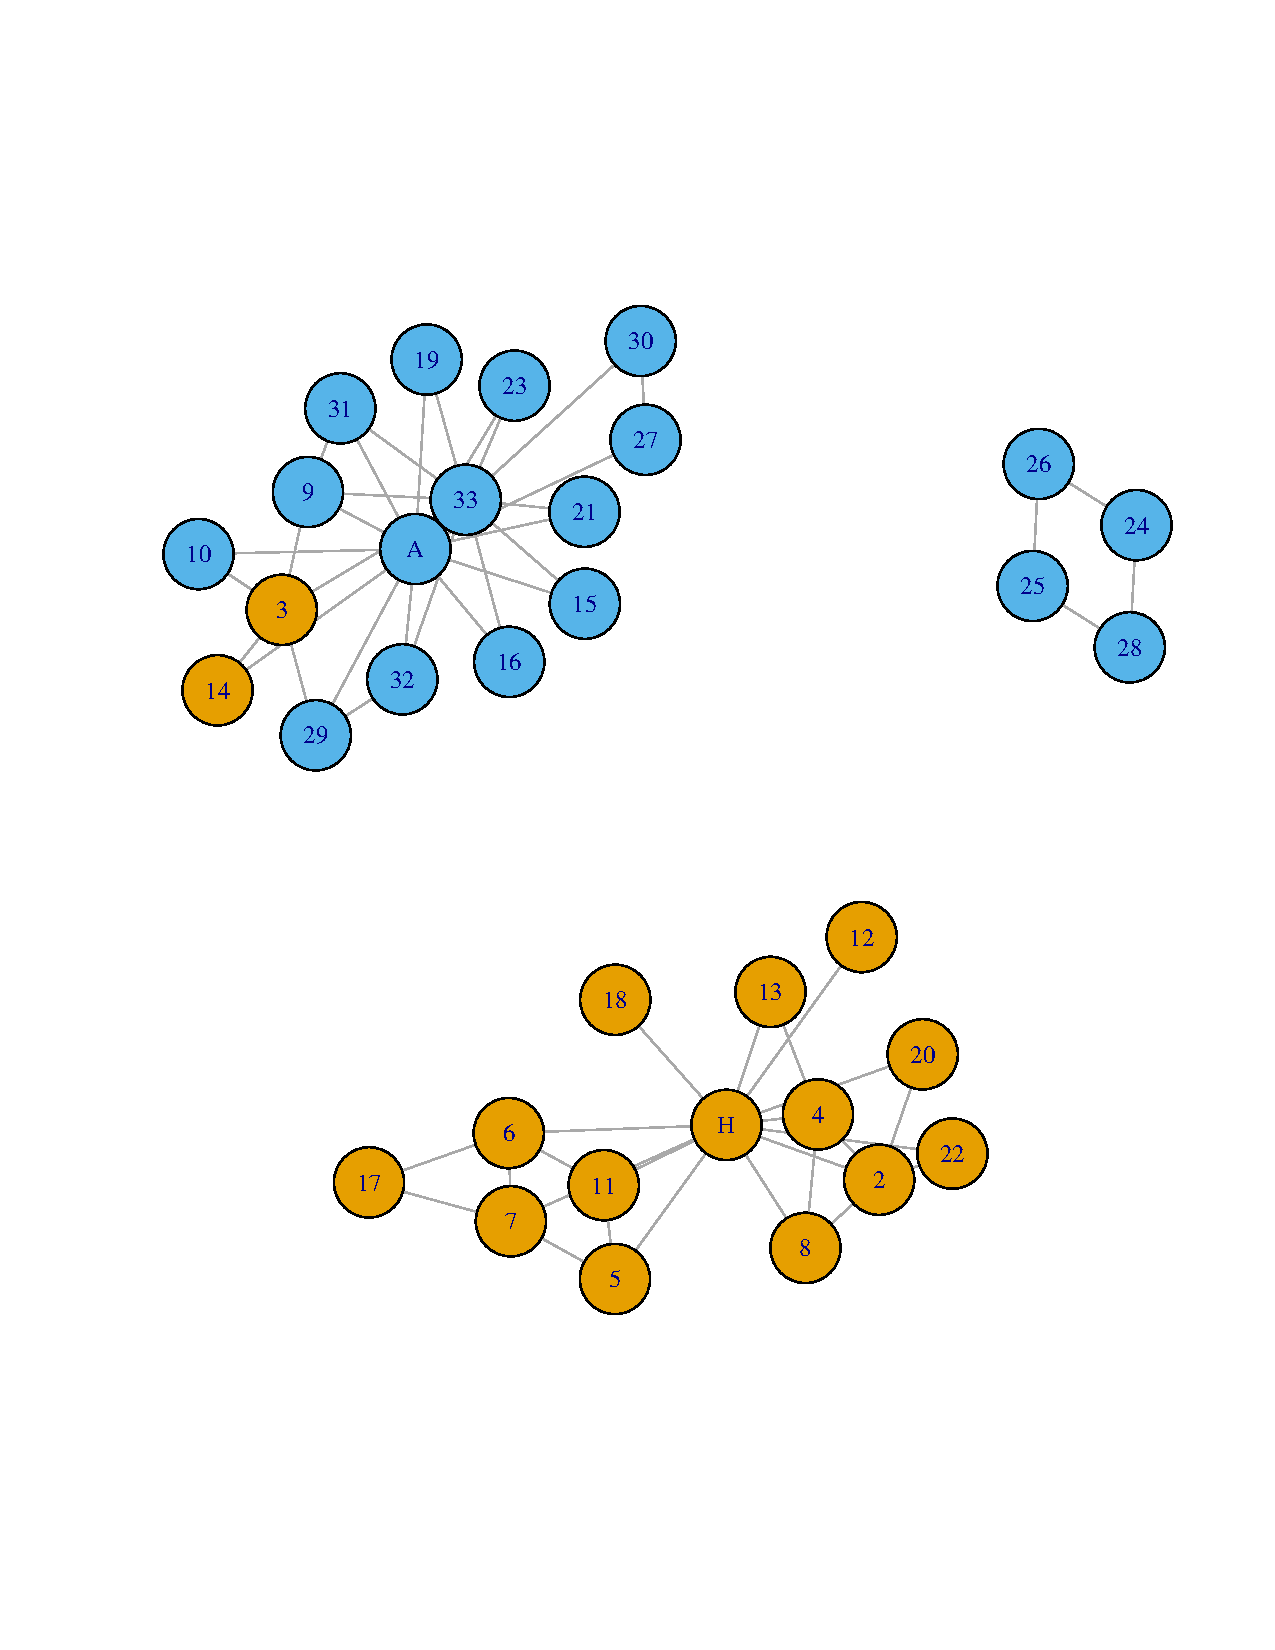
\includegraphics[scale=0.6]{predictedSplit3.pdf}
% \caption{Group split of 3 with Girvan-Newman algorithm from karateClub.R}
% \label{fig:split3}
% \end{figure}

\clearpage

\clearpage


% =================================
% Bibliography
% =================================

\begin{thebibliography}{9}
\bibitem{github}
Atkins, Grant. ``CS532 Assignment 9 Repository'' Github. N.p., 23 March 2017. Web. 23 March 2017.\url{https://github.com/grantat/cs532-s17/tree/master/assignments/A9}.
\bibitem{collectiveIntell}
Segaran, Toby. ``Programming Collective Intelligence''. O' Reilly, 2007. Web. 6 April 2017. \url{http://shop.oreilly.com/product/9780596529321.do}.
\bibitem{realmref}
``Realm now has an RSS feed''. Realm, 24 Oct 2014. Web. 30 April 2017. \url{https://news.realm.io/news/realm-rss-feed/}.
\end{thebibliography}

\end{document}